% ==============================================================================
% Proyecto integrador de Inteligencia de Negocios -- sustentación
% Maestría en Ciencias de la Información y las Comunicaciones (MCIC)
% Universidad Distrital Francisco José de Caldas
% ==============================================================================
\documentclass[aspectratio=169,10pt]{beamer}

\usepackage{fontspec}
\usepackage[spanish,es-noshorthands,es-tabla,es-nodecimaldot]{babel}
\usepackage{graphicx}
\usepackage{tikz}
\usepackage{booktabs}
\usepackage{array}
\usetikzlibrary{calc,positioning,arrows.meta,fit}

% Tipografía institucional: Cambria (títulos) y Times New Roman (texto)
\newfontfamily\cambriafont{cambria.ttc}[Path=../fuentes/, BoldFont=cambriab.ttf, ItalicFont=cambriai.ttf, BoldItalicFont=cambriaz.ttf]
\setmainfont{times.ttf}[Path=../fuentes/, BoldFont=timesbd.ttf, ItalicFont=timesi.ttf, BoldItalicFont=timesbi.ttf]
\setsansfont{times.ttf}[Path=../fuentes/, BoldFont=timesbd.ttf, ItalicFont=timesi.ttf, BoldItalicFont=timesbi.ttf]

% Paleta institucional
\definecolor{UDRed}{HTML}{ED3237}
\definecolor{UDDarkRed}{HTML}{A61C22}
\definecolor{UDGold}{HTML}{B49739}
\definecolor{UDBlue}{HTML}{1291C0}
\definecolor{UDGreen}{HTML}{00A859}
\definecolor{UDDarkGreen}{HTML}{047857}
\definecolor{UDSilver}{HTML}{64748B}
\definecolor{UDSable}{HTML}{373435}
\definecolor{UDLightGray}{HTML}{F8FAFC}
\definecolor{UDBorder}{HTML}{CBD5E1}

\setbeamertemplate{navigation symbols}{}
\setbeamersize{text margin left=3.15cm, text margin right=0.75cm}
\setbeamercolor{normal text}{fg=UDSable}
\setbeamercolor{itemize item}{fg=UDRed}
\setbeamercolor{enumerate item}{fg=UDRed}
\setbeamertemplate{itemize item}{\small$\blacktriangleright$}
\setbeamertemplate{enumerate item}{\insertenumlabel.}

\makeatletter
\setbeamertemplate{frametitle}{
  \vspace{0.45cm}
  \begin{minipage}{\textwidth}
    {\cambriafont\fontsize{14pt}{16pt}\selectfont\bfseries\color{UDSable}\insertframetitle\par}
    \ifx\insertframesubtitle\@empty\else
      \vskip2pt
      {\cambriafont\fontsize{8.5pt}{10pt}\selectfont\bfseries\color{UDRed}\insertframesubtitle\par}
    \fi
  \end{minipage}
}
\makeatother

% Número de página anclado a la esquina inferior derecha, dentro del área visible
\setbeamertemplate{footline}{%
  \ifnum\thepage>1
    \begin{tikzpicture}[remember picture,overlay]
      \node[anchor=south east, inner sep=0pt, text=UDSilver, font=\fontsize{7pt}{8pt}\selectfont]
        at ([xshift=-0.75cm, yshift=0.35cm]current page.south east) {\insertframenumber\,/\,\inserttotalframenumber};
    \end{tikzpicture}%
  \fi
}

\setbeamertemplate{background}{
\includegraphics[width=\paperwidth,height=\paperheight]{assets/fondo_contenido.jpg}}

\newcommand{\UDCard}[3]{%
  \begin{tikzpicture}
    \node[fill=#1, draw=#2, rounded corners=3pt, line width=0.7pt, inner sep=6pt, text width=\linewidth-14pt] {#3};
  \end{tikzpicture}%
}
\newcommand{\cardtitle}[2]{{\cambriafont\bfseries\color{#1}#2}\par\vspace{0.08cm}}
\newcommand{\decision}[1]{\UDCard{UDRed!6}{UDRed!60}{\footnotesize{\cambriafont\bfseries\color{UDRed}Decisión:} #1}}

\tikzset{
  paso/.style={draw=UDBorder, fill=white, rounded corners=2.5pt, line width=0.6pt, align=center,
               font=\fontsize{7.5pt}{9pt}\selectfont, inner sep=3pt, minimum height=1.0cm, text width=1.75cm},
  flecha/.style={thick, color=UDRed, -{Latex[length=2mm]}},
}

\begin{document}

% ------------------------------------------------------------------ portada
{
\setbeamertemplate{background}{}
\begin{frame}[plain]
  \begin{tikzpicture}[remember picture,overlay]
    \node[anchor=south west,inner sep=0pt] at (current page.south west)
      {
\includegraphics[width=\paperwidth,height=\paperheight]{assets/portada_base.jpg}};
    \node[anchor=north west, align=left, inner sep=0pt] at ([xshift=8.10cm, yshift=-2.60cm]current page.north west) {
      \begin{minipage}{5.2cm}\raggedright\hyphenpenalty=10000
        {\cambriafont\fontsize{12pt}{14pt}\selectfont\bfseries\color{UDSable}¿En qué invertir para crecer el próximo año?\par}
        \vspace{0.06cm}
        {\cambriafont\fontsize{7.5pt}{9pt}\selectfont\bfseries\color{UDRed}Proyecto integrador de Inteligencia de Negocios\par}
        \vspace{0.05cm}
        {\color{UDRed}\rule{5.0cm}{1.0pt}\par}
        \vspace{0.06cm}
        {\cambriafont\fontsize{7.5pt}{9pt}\selectfont\bfseries\color{UDSable}Juan Felipe Rodríguez Galindo\par}
        {\fontsize{6.4pt}{7.4pt}\selectfont\color{UDSilver}20261595004\par}
        {\cambriafont\fontsize{7.5pt}{9pt}\selectfont\bfseries\color{UDSable}Carlos Stiven Mora Hoyos\par}
        {\fontsize{6.4pt}{7.4pt}\selectfont\color{UDSilver}20261595003\par}
        \vspace{0.05cm}
        {\fontsize{6.4pt}{7.6pt}\selectfont\color{UDSable}Maestría en Ciencias de la Información y las Comunicaciones\par}
        {\fontsize{6.4pt}{7.6pt}\selectfont\color{UDBlue}2026\par}
      \end{minipage}
    };
  \end{tikzpicture}
\end{frame}
}

% ------------------------------------------------------------------ 2
\begin{frame}{La decisión}{Cuatro iniciativas compiten por el presupuesto del próximo año}
  \begin{columns}[T,onlytextwidth]
    \begin{column}{0.48\textwidth}
      \UDCard{white}{UDBorder}{\cardtitle{UDBlue}{Embudo mejorado}
        {\small Llevar a toda la web la página, el botón, el descargable y el pago simplificado que ya se probaron.}}
      \vspace{0.15cm}
      \UDCard{white}{UDBorder}{\cardtitle{UDGold!90!black}{Webinars}
        {\small Invitar a los contactos que ya conocen la marca.}}
    \end{column}
    \begin{column}{0.48\textwidth}
      \UDCard{white}{UDBorder}{\cardtitle{UDRed}{Duplicar publicidad}
        {\small Doblar el gasto diario en Facebook y Google.}}
      \vspace{0.15cm}
      \UDCard{white}{UDBorder}{\cardtitle{UDDarkGreen}{Producto nuevo}
        {\small Ofrecer un producto premium, más caro.}}
    \end{column}
  \end{columns}
  \vspace{0.3cm}
  \UDCard{UDLightGray}{UDRed!60}{\small Todo se mide en \textbf{contribución}: lo que queda de la venta después de
  pagar el producto, la publicidad atribuida y el despacho. Una venta que cuesta más de lo que deja sube los
  ingresos y aun así pierde dinero.}
  \note{Tenemos cuatro opciones y hay que elegir. La pregunta no es cuál vende más sino cuál deja más contribución
  y con qué riesgo.}
\end{frame}

% ------------------------------------------------------------------ datos
\begin{frame}{Qué datos tenemos}{20.000 filas: cada fila es una persona interesada en comprar (una oportunidad)}
  \begin{columns}[T,onlytextwidth]
    \begin{column}{0.50\textwidth}
      \footnotesize\setlength{\tabcolsep}{3pt}
      \begin{tabular*}{\linewidth}{@{}l@{\extracolsep{\fill}}l@{}}
        \toprule
        Pregunta & Columnas \\
        \midrule
        ¿Quién es? & segmento, país, dispositivo \\
        ¿Por dónde llegó? & canal, campaña, nivel de pauta \\
        ¿Qué vio? & página, botón, webinar, oferta \\
        ¿Qué pasó? & compró o no, días al cierre \\
        ¿Cuánto valió? & ingreso, costo, contribución \\
        \bottomrule
      \end{tabular*}
      \vspace{0.15cm}

      {\footnotesize\color{UDSilver} 28 columnas, enero de 2024 a abril de 2026.}
    \end{column}
    \begin{column}{0.46\textwidth}
      \UDCard{UDLightGray}{UDBlue!60}{\cardtitle{UDBlue}{Una fila, como ejemplo: TX-000104}
        {\footnotesize 6 de enero de 2024. Cliente \textbf{Enterprise} de \textbf{España} que llegó por
        \textbf{Google Ads}. Vio la web de siempre y no fue a ningún webinar.\par\vspace{0.1cm}
        \textbf{Compró} a los 2 días por \textbf{€1.554,86}. Su publicidad costó €9,05.
        Contribución: \textbf{€1.076,01}.}}
    \end{column}
  \end{columns}
  \note{Aterrizar el dato: cuando hablemos de oportunidades, es esto. Usamos esta misma fila en la limpieza.}
\end{frame}

% ------------------------------------------------------------------ 3
\begin{frame}{Cómo trabajamos}{20.000 oportunidades, enero de 2024 a abril de 2026, datos sintéticos}
  \vspace{0.3cm}
  \begin{center}
  \begin{tikzpicture}[node distance=0.32cm]
    \node[paso] (a) {\textbf{CSV original}\\solo lectura};
    \node[paso, right=of a] (b) {\textbf{SQL}\\vista limpia y\\15 reglas};
    \node[paso, right=of b] (c) {\textbf{Estrella}\\2 hechos,\\5 dimensiones};
    \node[paso, right=of c] (d) {\textbf{Modelo}\\regresión\\logística};
    \node[paso, right=of d, fill=UDRed!8, draw=UDRed] (e) {\textbf{Simulación}\\bootstrap +\\Monte Carlo};
    \draw[flecha] (a) -- (b); \draw[flecha] (b) -- (c); \draw[flecha] (c) -- (d); \draw[flecha] (d) -- (e);
  \end{tikzpicture}
  \end{center}
  \vspace{0.35cm}
  \begin{columns}[T,onlytextwidth]
    \begin{column}{0.32\textwidth}
      \UDCard{white}{UDBorder}{\cardtitle{UDBlue}{Reproducible}{\footnotesize Todo se regenera con
        \texttt{make run}; cada cifra cita la vista o el archivo de origen.}}
    \end{column}
    \begin{column}{0.32\textwidth}
      \UDCard{white}{UDBorder}{\cardtitle{UDRed}{Sin fuga}{\footnotesize El modelo solo usa lo que se sabe antes
        de la venta.}}
    \end{column}
    \begin{column}{0.32\textwidth}
      \UDCard{white}{UDBorder}{\cardtitle{UDDarkGreen}{Validado}{\footnotesize El proceso se detiene si alguna
        regla o control de la estrella falla.}}
    \end{column}
  \end{columns}
\end{frame}

% ------------------------------------------------------------------ 4
\begin{frame}{Los datos tenían trampas}{Las reglas dan cero, pero eso no basta}
  \begin{columns}[T,onlytextwidth]
    \begin{column}{0.48\textwidth}
      \UDCard{white}{UDBorder}{\cardtitle{UDRed}{Costo fijo oculto}{\footnotesize Cada venta carga €22 de despacho
        que no aparecía en ninguna columna.}}
      \vspace{0.12cm}
      \UDCard{white}{UDBorder}{\cardtitle{UDRed}{Gasto que no se suma}{\footnotesize El gasto diario de campaña cambia en
        cada fila: indica el nivel de pauta, no un pago. Sumarlo daría €4,55 M sin sentido.}}
      \vspace{0.12cm}
      \UDCard{white}{UDBorder}{\cardtitle{UDRed}{Sin gasto total}{\footnotesize Solo el costo atribuido se puede sumar
        (€117 mil en pauta); el gasto real hay que pedirlo a finanzas.}}
    \end{column}
    \begin{column}{0.48\textwidth}
      \UDCard{white}{UDBorder}{\cardtitle{UDGold!90!black}{Producto para pocos}{\footnotesize Solo se ofreció a
        tres segmentos de ticket alto: hay que comparar dentro de cada uno.}}
      \vspace{0.12cm}
      \UDCard{white}{UDBorder}{\cardtitle{UDGold!90!black}{Datos del futuro}{\footnotesize Ingreso, margen y días de
        cierre quedan fuera del modelo.}}
      \vspace{0.12cm}
      \UDCard{white}{UDBorder}{\cardtitle{UDGold!90!black}{Cambios por épocas}{\footnotesize Pauta y embudo
        cambiaron por periodos; comparar promedios mezcla palanca y momento.}}
    \end{column}
  \end{columns}
  \note{Si ignoramos estos puntos llegamos a conclusiones equivocadas, aunque las validaciones den cero.}
\end{frame}

% ------------------------------------------------------------------ limpieza 1
\begin{frame}{Limpieza con un ejemplo: el costo oculto}{La misma fila TX-000104}
  \begin{columns}[c,onlytextwidth]
    \begin{column}{0.50\textwidth}
      \footnotesize\setlength{\tabcolsep}{3pt}
      \begin{tabular*}{\linewidth}{@{}l@{\extracolsep{\fill}}r@{}}
        \toprule
        Utilidad bruta (€1.554,86 × 71,2 \%) & €1.107,06 \\
        $-$ Publicidad atribuida & €9,05 \\
        \midrule
        Debería quedar & €1.098,01 \\
        El archivo dice & €1.076,01 \\
        \midrule
        \textbf{Diferencia} & \textbf{€22,00} \\
        \bottomrule
      \end{tabular*}
    \end{column}
    \begin{column}{0.46\textwidth}
      \UDCard{white}{UDBorder}{\footnotesize Pasa en las \textbf{2.096 ventas}, siempre €22, y nunca en las filas
        sin venta. No es un error: es un \textbf{costo fijo por venta} (despacho).}
      \vspace{0.15cm}
      \decision{lo volvimos regla de validación y lo descontamos en todos los escenarios.}
    \end{column}
  \end{columns}
  \note{Lo encontramos porque la regla de contribución fallaba. Al entenderlo, se convirtió en regla.}
\end{frame}

% ------------------------------------------------------------------ limpieza 2
\begin{frame}{Limpieza con un ejemplo: el gasto que no se suma}{Facebook Ads, 23 de junio de 2025: llegaron 14 personas}
  \begin{columns}[c,onlytextwidth]
    \begin{column}{0.50\textwidth}
      \UDCard{white}{UDBorder}{\footnotesize Cada una de las 14 filas trae un ``gasto diario'' \textbf{distinto},
        entre €993 y €1.164. Indica qué tan fuerte era la pauta, no cuánto se pagó.}
      \vspace{0.15cm}
      \UDCard{UDRed!6}{UDRed!60}{\footnotesize Sumar las 14 filas: \textbf{€15.071}, una cifra sin sentido.\par
        En todo el archivo daría \textbf{€4,55 M}.}
    \end{column}
    \begin{column}{0.46\textwidth}
      \UDCard{UDLightGray}{UDDarkGreen!60}{\footnotesize Lo único que se puede sumar ese día es el
        \textbf{costo atribuido}: \textbf{€328}.}
      \vspace{0.15cm}
      \decision{el gasto diario solo se promedia (tabla aparte en la estrella); el gasto real se le pide a
        finanzas.}
    \end{column}
  \end{columns}
  \note{Probamos la regla ``un gasto por canal y día'' y falló en 7.764 de 7.868 filas pagadas: por eso no es un
  pago repetido.}
\end{frame}

% ------------------------------------------------------------------ limpieza 3
\begin{frame}{Limpieza con un ejemplo: ceros que no son errores}{El 90 \% de las oportunidades no compró}
  \begin{columns}[c,onlytextwidth]
    \begin{column}{0.50\textwidth}
      \footnotesize\setlength{\tabcolsep}{3pt}
      \begin{tabular*}{\linewidth}{@{}l@{\extracolsep{\fill}}r@{}}
        \toprule
        Ticket promedio & \\
        \midrule
        Sobre todas las filas & €116 \\
        Sobre las ventas & \textbf{€1.110} \\
        \bottomrule
      \end{tabular*}
      \vspace{0.2cm}

      {\footnotesize Sin venta, el ticket es 0 porque no compró, no porque falte el dato.}
    \end{column}
    \begin{column}{0.46\textwidth}
      \UDCard{white}{UDBorder}{\cardtitle{UDGold!90!black}{Datos del futuro}{\footnotesize Ingreso, margen y días
        de cierre solo se conocen \textbf{después} de comprar. Usarlos para predecir la compra sería hacer trampa.}}
      \vspace{0.15cm}
      \decision{el ticket se calcula solo sobre ventas, y esas columnas quedan fuera del modelo.}
    \end{column}
  \end{columns}
\end{frame}

% ------------------------------------------------------------------ procesos
\begin{frame}{Para qué sirvió cada proceso}{Cada paso responde una pregunta y alimenta una decisión}
  \footnotesize\setlength{\tabcolsep}{4pt}
  \begin{tabular*}{\linewidth}{@{}>{\bfseries}l@{\extracolsep{\fill}}p{3.6cm}p{3.4cm}p{3.6cm}@{}}
    \toprule
    \normalfont Proceso & Qué es & Pregunta & Decisión que permitió \\
    \midrule
    Limpiar & Vista SQL y 15 reglas & ¿Podemos confiar en el dato? & Corregir costos y no sumar el gasto diario \\
    Organizar & Esquema estrella: hechos y dimensiones & ¿Cómo cortar sin errores? & Comparar canales, meses y clientes \\
    Medir & Indicadores (KPI) & ¿Cómo va el negocio? & Dejar de crecer con pauta \\
    Predecir & Regresión logística & ¿Qué hace que alguien compre? & Medir asistentes; priorizar por puntaje \\
    Simular & \textit{Bootstrap} + Monte Carlo & ¿Cuánto gana y arriesga cada opción? & Embudo ahora, producto en piloto \\
    \bottomrule
  \end{tabular*}
  \note{Los siguientes slides muestran cada decisión con su evidencia.}
\end{frame}

% ------------------------------------------------------------------ kpi
\begin{frame}{Los indicadores que usamos}{Último año: mayo de 2025 a abril de 2026}
  \footnotesize\setlength{\tabcolsep}{4pt}
  \begin{tabular*}{\linewidth}{@{}l@{\extracolsep{\fill}}llr@{}}
    \toprule
    Indicador & Pregunta & Cálculo & Último año \\
    \midrule
    Conversión & ¿Cuántos compran? & ventas ÷ oportunidades & 12,2 \% \\
    Ticket medio & ¿Cuánto vale una venta? & ingresos ÷ ventas & €1.142 \\
    Costo por venta & ¿Cuánto cuesta conseguirla? & costo atribuido ÷ ventas & €66 \\
    ROAS & ¿Cuánto deja cada euro de pauta? & ingresos ÷ costo atribuido & 17,2 \\
    \textbf{Contribución por oportunidad} & ¿Cuánto vale cada interesado? & contribución ÷ oportunidades & \textbf{€93} \\
    Adopción del embudo & ¿Cuántos ven la web nueva? & con las 4 mejoras ÷ total & 19 \% \\
    \bottomrule
  \end{tabular*}
  \vspace{0.25cm}

  {\footnotesize\color{UDSilver} Fuente: \texttt{salidas/crecimiento.csv}; adopción contada sobre la vista
  \texttt{ventas} (24 \% en 2026).}
  \note{El más útil es la contribución por oportunidad: junta en un número si compran, cuánto pagan y cuánto
  costó traerlos.}
\end{frame}

% ------------------------------------------------------------------ 5
\begin{frame}{El negocio crece vendiendo mejor}{Últimos 12 meses frente a los 12 anteriores}
  \begin{columns}[c,onlytextwidth]
    \begin{column}{0.42\textwidth}
      \footnotesize\setlength{\tabcolsep}{3pt}
      \begin{tabular*}{\linewidth}{@{}l@{\extracolsep{\fill}}r r@{}}
        \toprule
        & Anterior & Último \\
        \midrule
        Ventas & 694 & 1.224 \\
        Conversión & 9,0 \% & 12,2 \% \\
        Costo por venta & €81 & €66 \\
        Contribución & €487 mil & \textbf{€934 mil} \\
        \bottomrule
      \end{tabular*}
      \vspace{0.25cm}

      \UDCard{UDLightGray}{UDGold!80}{\footnotesize El embudo explica parte del salto, no todo: en julio de 2025 la
      conversión ya había subido sin embudo completo, justo cuando terminó la pauta saturada.}
      \vspace{0.12cm}
      \decision{extender el embudo (hoy lo ve una de cada cuatro), con grupo de control.}
    \end{column}
    \begin{column}{0.54\textwidth}
      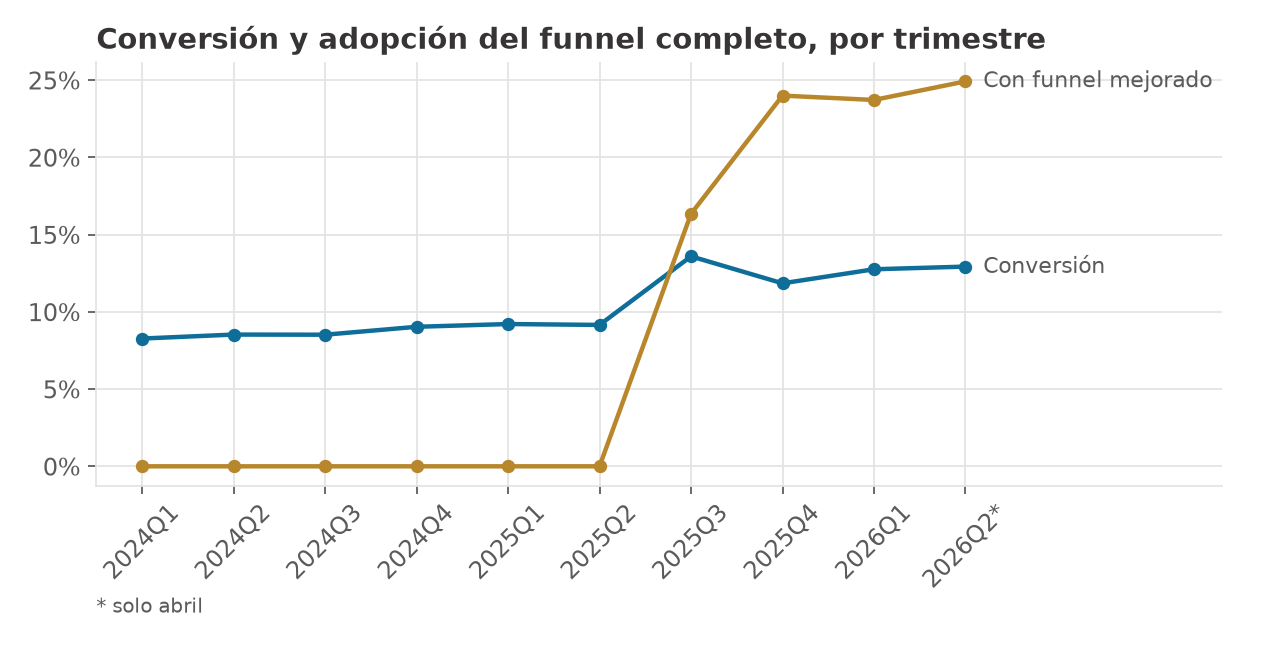
\includegraphics[width=\linewidth]{../informe/fig/2_tendencia_funnel.png}
    \end{column}
  \end{columns}
  \note{Contribución +92 \%. La conversión sube en 2025T3 con el embudo, pero el dato mensual muestra otro cambio a la
  vez; por eso recomendamos medirlo con grupo de control.}
\end{frame}

% ------------------------------------------------------------------ 6
\begin{frame}{Más publicidad, peor resultado}{Facebook y Google: 39 \% de las oportunidades, 13 \% de la contribución}
  \begin{center}
    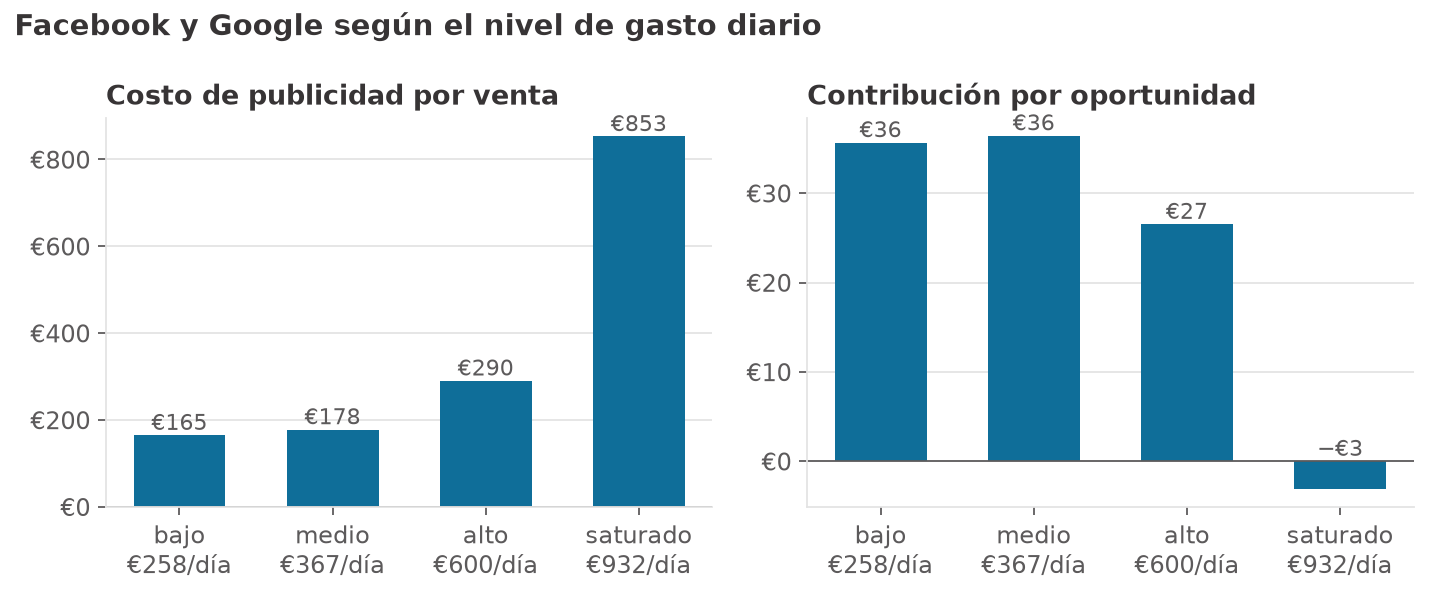
\includegraphics[width=0.80\linewidth]{../informe/fig/3_ads_saturacion.png}
  \end{center}
  \vspace{-0.1cm}
  {\small Con gasto saturado, cada venta cuesta casi cinco veces más y cada oportunidad pierde dinero: llegan más
  interesados, pero de peor calidad (puntaje 52,5 → 37,8).}
  \vspace{0.1cm}

  \decision{no duplicar la publicidad.}
\end{frame}

% ------------------------------------------------------------------ 7
\begin{frame}{¿Qué hace que alguien compre?}{Regresión logística entrenada con 2024--2025 y evaluada en 2026}
  \begin{columns}[c,onlytextwidth]
    \begin{column}{0.54\textwidth}
      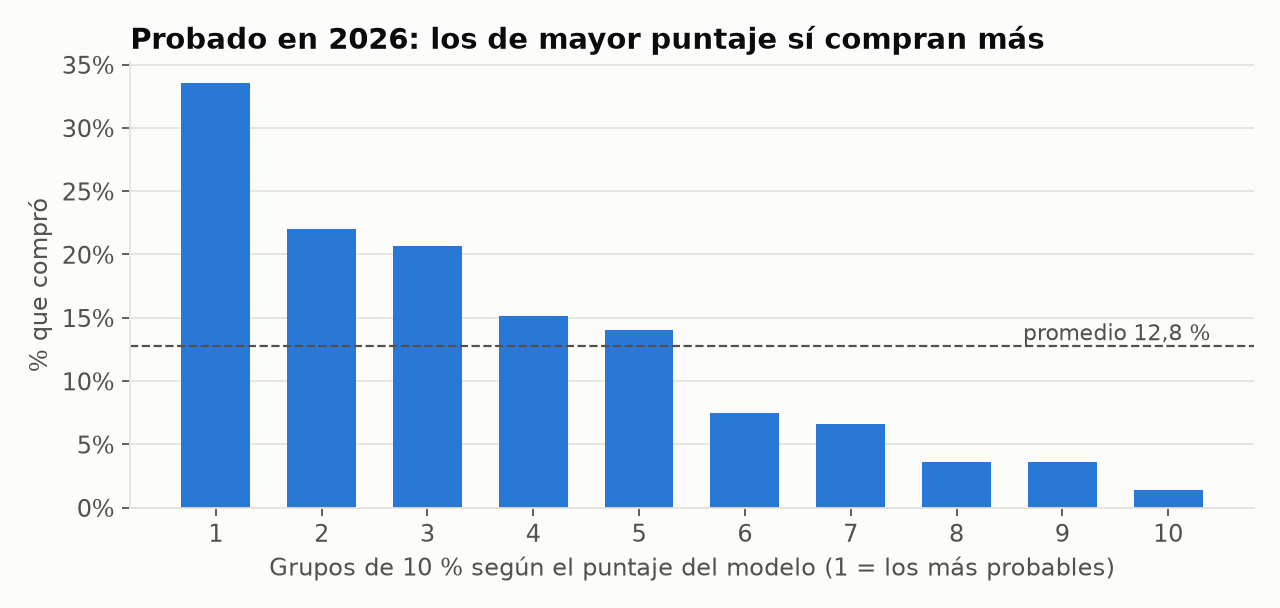
\includegraphics[width=\linewidth]{../informe/fig/4_lift_modelo.png}
      \vspace{0.05cm}
      {\footnotesize AUC 0,745. El 20 \% con mayor puntaje concentra el 43 \% de las ventas.}
    \end{column}
    \begin{column}{0.42\textwidth}
      \footnotesize\setlength{\tabcolsep}{4pt}
      \begin{tabular*}{\linewidth}{@{}l@{\extracolsep{\fill}}r@{}}
        \toprule
        Factor & Chances \\
        \midrule
        Puntaje previo (+1 desv.) & +82 \% \\
        Asistir al webinar & +43 \% \\
        Botón de beneficio & +24 \% \\
        Página nueva & +17 \% \\
        Material descargable & +16 \% \\
        Pauta saturada (vs. media) & $-$49 \% \\
        Oferta de producto nuevo & $-$38 \% \\
        \bottomrule
      \end{tabular*}
      \vspace{0.15cm}

      \decision{llamar primero a los de mayor puntaje; en webinars, medir asistentes y no invitados.}
    \end{column}
  \end{columns}
  \note{Elegimos un modelo explicable porque lo usamos para comparar escenarios, no para ganar en precisión.}
\end{frame}

% ------------------------------------------------------------------ 8
\begin{frame}{Comparación de las cuatro iniciativas}{200 réplicas bootstrap × 10.000 simulaciones de costo y alcance}
  \begin{center}
    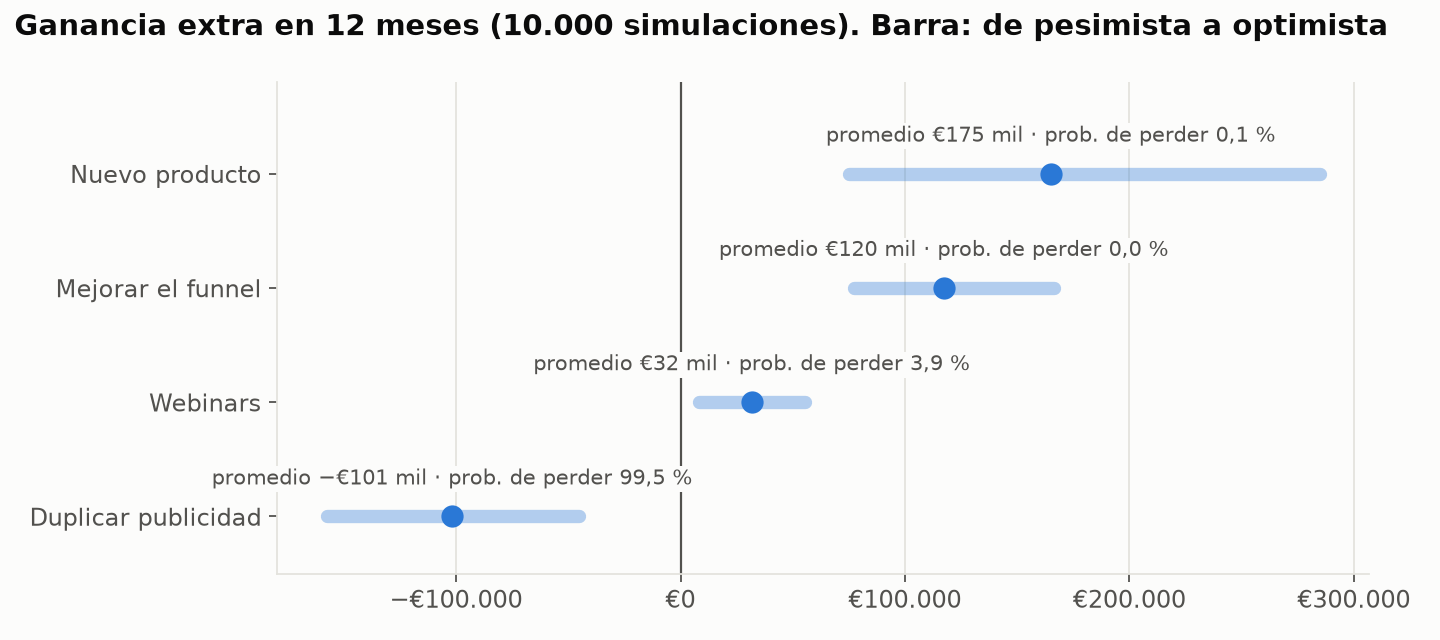
\includegraphics[width=0.88\linewidth]{../informe/fig/5_montecarlo.png}
  \end{center}
  {\small Ninguna iniciativa sale como se planea: costo y alcance varían. Por eso probamos cada una 10.000 veces
  con supuestos distintos. El punto es el valor esperado; la barra va del escenario pesimista (P10) al optimista
  (P90).}
  \note{Es como lanzar el dado muchas veces para ver todos los resultados posibles, no solo uno.}
\end{frame}

% ------------------------------------------------------------------ simulación -> decisión
\begin{frame}{De la simulación a la decisión}{Contribución adicional a doce meses}
  \footnotesize\setlength{\tabcolsep}{4pt}
  \begin{tabular*}{\linewidth}{@{}l@{\extracolsep{\fill}}rrl@{}}
    \toprule
    Iniciativa & Esperado & P(pérdida) & Lectura \\
    \midrule
    Producto nuevo & €175 mil & 0,1 \% & Gana más, pero con solo 55 ventas de evidencia \\
    Embudo mejorado & €120 mil & 0,0 \% & Gana bien, rango estrecho, mejor retorno por euro \\
    Webinars & €32 mil & 3,9 \% & Gana poco; solo si cuesta menos de €48 mil al año \\
    Duplicar publicidad & $-$€101 mil & 99,5 \% & Pierde casi siempre \\
    \bottomrule
  \end{tabular*}
  \vspace{0.3cm}

  \decision{embudo ahora, por ser la apuesta más segura; producto en piloto, por ser la más incierta.}
  \note{Fuente: salidas/montecarlo\_resumen.csv. El embudo y el producto no compiten: uno sube la conversión y el
  otro el valor por venta.}
\end{frame}

% ------------------------------------------------------------------ 9
\begin{frame}{Qué tan firmes son estos números}{Las probabilidades de pérdida suponen que el modelo es correcto}
  \begin{columns}[T,onlytextwidth]
    \begin{column}{0.48\textwidth}
      \UDCard{white}{UDBorder}{\cardtitle{UDRed}{Producto: 55 ventas}{\footnotesize Se extrapola a diez veces más
        oportunidades. Los €175 mil son un techo optimista.}}
      \vspace{0.12cm}
      \UDCard{white}{UDBorder}{\cardtitle{UDRed}{No son experimentos}{\footnotesize Al webinar asiste quien quiere,
        y a los invitados se les eligió con mejor puntaje.}}
    \end{column}
    \begin{column}{0.48\textwidth}
      \UDCard{white}{UDBorder}{\cardtitle{UDGold!90!black}{Rangos optimistas}{\footnotesize El bootstrap remuestrea
        filas sueltas e ignora las épocas; por bloques, los rangos serían más anchos.}}
      \vspace{0.12cm}
      \UDCard{white}{UDGold!80}{\cardtitle{UDGold!90!black}{Umbrales}{\footnotesize Si el producto cuesta más de
        €84 mil, gana el embudo. Los webinars solo compensan por debajo de €48 mil al año.}}
    \end{column}
  \end{columns}
  \note{Cerramos con los límites: una recomendación que no dice cuándo deja de valer no se puede defender.}
\end{frame}

% ------------------------------------------------------------------ 10
\begin{frame}{Recomendación}{El embudo y el producto no compiten: uno sube la conversión, el otro el valor por venta}
  \begin{columns}[T,onlytextwidth]
    \begin{column}{0.48\textwidth}
      \UDCard{UDLightGray}{UDBlue!60}{\cardtitle{UDBlue}{Hacer ahora}
        \begin{enumerate}\footnotesize\setlength{\itemsep}{0.1cm}
          \item Extender el embudo mejorado (hoy lo ve una de cada cuatro oportunidades), con grupo de control.
          \item Usar el puntaje del modelo para priorizar la atención comercial.
        \end{enumerate}}
      \vspace{0.12cm}
      \UDCard{UDLightGray}{UDRed!60}{\cardtitle{UDRed}{No hacer}
        {\footnotesize Duplicar la publicidad. Antes, conseguir con finanzas el gasto real de pauta.}}
    \end{column}
    \begin{column}{0.48\textwidth}
      \UDCard{UDLightGray}{UDGold!80}{\cardtitle{UDGold!90!black}{Probar primero}
        \begin{enumerate}\footnotesize\setlength{\itemsep}{0.1cm}
          \item Piloto del producto un trimestre, con oferta al azar en B2B Services, Ecommerce y Enterprise.
          \item Webinars solo si cuestan menos de €48 mil al año; medir asistentes, no invitados.
        \end{enumerate}}
      \vspace{0.12cm}
      {\footnotesize\color{UDSilver} Datos sintéticos: el método se puede reutilizar, las cifras no describen una
      empresa real.}
    \end{column}
  \end{columns}
\end{frame}

% ------------------------------------------------------------------ cierre
{
\setbeamertemplate{background}{}
\begin{frame}[plain]
  \begin{tikzpicture}[remember picture,overlay]
    \node[anchor=south west,inner sep=0pt] at (current page.south west)
      {
\includegraphics[width=\paperwidth,height=\paperheight]{assets/cierre_base.jpg}};
    \node[anchor=center, fill=white, fill opacity=0.94, text opacity=1, rounded corners=4pt, inner sep=14pt,
          line width=0.8pt, draw=UDBorder] at ([xshift=3.2cm, yshift=0.2cm]current page.center) {
      \begin{minipage}{5.8cm}
        \centering
        {\cambriafont\fontsize{16pt}{18pt}\selectfont\bfseries\color{UDRed}Gracias\par}
        \vspace{0.2cm}
        {\cambriafont\fontsize{10.5pt}{13pt}\selectfont\bfseries\color{UDSable}Preguntas y discusión\par}
        \vspace{0.2cm}
        {\color{UDRed}\rule{4.2cm}{1.2pt}\par}
        \vspace{0.2cm}
        {\cambriafont\fontsize{9pt}{11pt}\selectfont\bfseries\color{UDSable}Juan Felipe Rodríguez Galindo\par}
        {\cambriafont\fontsize{9pt}{11pt}\selectfont\bfseries\color{UDSable}Carlos Stiven Mora Hoyos\par}
        \vspace{0.08cm}
        {\fontsize{8pt}{10pt}\selectfont\color{UDSable}Maestría en Ciencias de la Información\\y las Comunicaciones\par}
        \vspace{0.06cm}
        {\fontsize{7.5pt}{9pt}\selectfont\color{UDSilver}Inteligencia de Negocios\par}
      \end{minipage}
    };
  \end{tikzpicture}
\end{frame}
}

\end{document}
